% !TeX root = ../thesis.tex

\chapter{Related Work}
\label{sec:related-work}

The presented work is inspired by multiple research fields. This chapter provides a brief overview on literature for these topics.


\section{Semantic Segmentation}

Semantic segmentation has widespread applications in medicine, industry as well as in mobile systems for semantic scene segregation. Semantic segmentation is a task of assigning class label to each pixel in a target image. Figure \ref{fig:rgb_semseg} shows an RGB image from Cityscapes dataset \cite{Cordts2015} and corresponding semantic segmentation output. Traditionally, semantic segmentation approaches relied on low-level cues like gradients, contours, contrasts and pixel relationships. Some of the successful earlier segmentation approaches are \textit{semantic texton forests} that applied decision tree ensembles at pixel level. Such random forest  based algorithm were usually coupled with noise reduction unary terms  \cite{Shotton2008}, \cite{Sturgess2009}. Significant improvements have been made in past decade since the deep learning methods were adopted for semantic segmentation task. One of the earlier approaches include \cite{Ciresan2012}, that tackled the problem of semantic segmentation of neuron membrane in electron microscopy images.


\begin{figure}[!htb]
    \subfigure[ RGB Image]{
        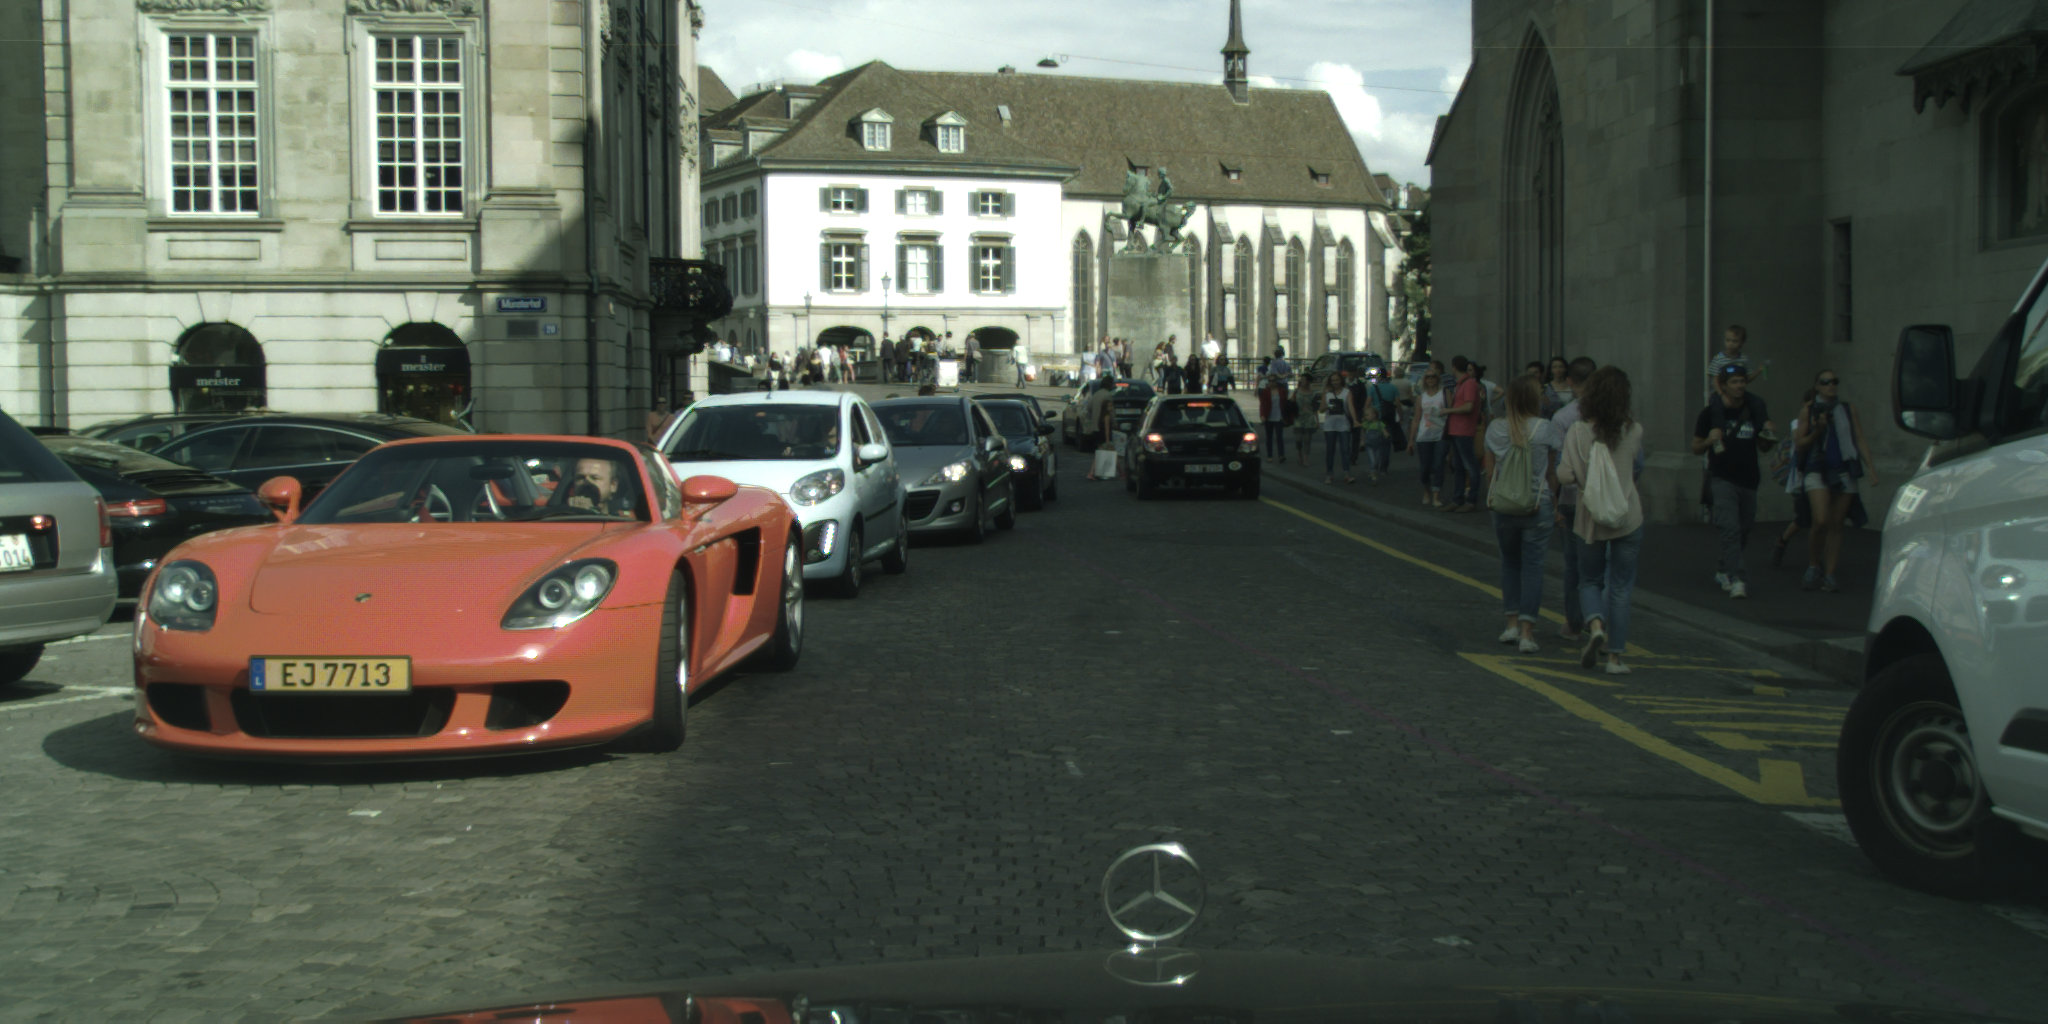
\includegraphics[width = \textwidth / 2 ]{Graphics/Related_Work/zurich_000068_000019_leftImg8bit}
        \label{fig:rgb_image}}
    \subfigure[Semantic Segmentation]{
        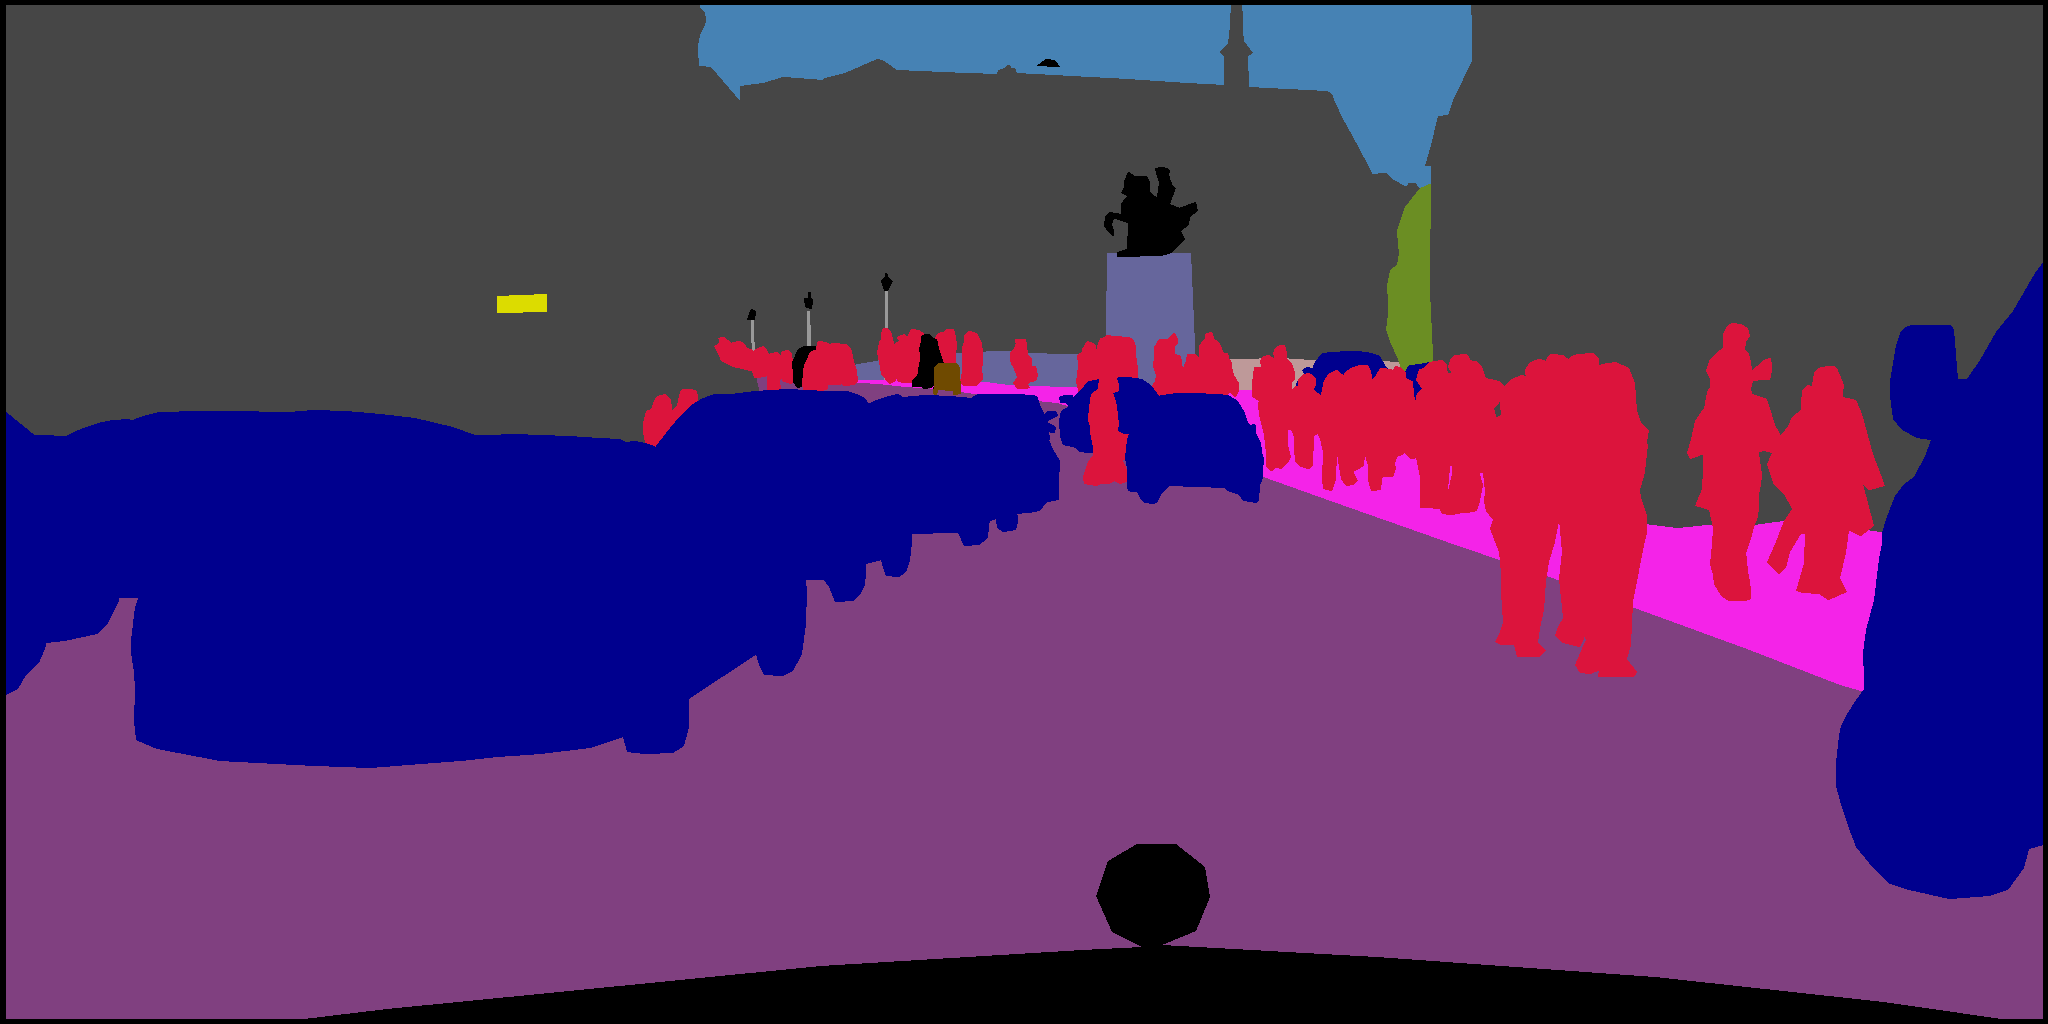
\includegraphics[width = \textwidth / 2 ]{Graphics/Related_Work/zurich_000068_000019_gtFine_color}
        \label{fig:semseggtfine}}
    \caption[RGB Image and Semantic Segmentation]{Illustration of an RGB Image taken from drivers perspective and its corresponding semantic segmentation taken from Cityscapes Dataset a) RGB Image b) semantic segmentation \cite{Cordts2015}}
    \label{fig:rgb_semseg}
\end{figure}

Recurrent neural networkss (RNNs) were used to capturing long range pixel dependencies in images for semantic segmentation. Although, it outperformed traditional methods however, boundaries were not preserved \cite{Pinheiro2014}. Significant improvements were made using end-to-end trained, fully convolutional networks (FCN), that relied on transpose convolutional layer to cop with sparse predictions and boundry preservance as faced by earlier approaches \cite{Long2015}. A similar FCN based approach was proposed that used deconvolutional layers to gradually regenerate the original resolution while maintaining boundries \cite{Noh2015}. 
 
 Since then, a huge number of publications relied on FCN architectures to solve the problem of pixel-wise semantic segmentation. Improvement in various areas of semantic segmentation were made to tweak and enhance performance in various aspects. DeepLab, used a combination of a FCN with upsampled convolutions and fully connected conditional random fields (CRFs) to improve localization performance in semantic segmentation tasks \cite{Chen2018}. They also show that atrous convolutions as explained in chapter \ref{sec:fundamentals} are helpful in explicitly controlling the field of view of convolutional filters.
 CRFs are however a post-processing step which was replaced with an encoder-decoder structure, where low-level features from lower layers were fed into higher-level layers to re-generate better boundaries \cite{Deeplabv3+:journals/corr/abs-1802-02611}. Other successful encoder-decoder structure based semantic segmentation approache was U-Net \cite{Ronneberger2015}. A later improved version is Unet++, where the encoder and decoder sub-networks are connected through a series of nested, dense skip pathways \cite{Zhou2018}.

\section{Instance Segmentation}
Instance segmentation is one of the most challenging tasks in computer vision, since it requires segmentation of all individual instances of predefined set of classes. Instance segmentation essentially requires solving object detection and semantic segmentation task simultaneously because it is desired to predict the right class label for pixels and also extent of each instance by masking it. Difference between semantic segmentation and instance segmentation has been illustrated in the figure \ref{fig:rgb_instsemseg}.

Earlier instance segmentation methods like \textit{simultaneous detection and segmentation} (SDS) \cite{Hariharan2014}, used a bottom up region proposal based approaches to score proposed regions with class labels to produce instance segmentation results. Those region proposals relied mostly on \textit{selective search} \cite{Uijlings2013} or  \textit{multi-scale combinatorial grouping} (MCG) \cite{Arbelaez2014} that extract possible coherent regions and groups them to generate multi-scale region proposals. These class agnostic proposals were scored using of \textit{Regional - Convolutional Neural Networks} (R-CNNs) based object detection algorithms \cite{Girshick2014} and its successor \textit{Fast- RCNN} \cite{Girshick2015}. Fast R-CNN is an improved verion of vanilla R-CNN that removed redundant computations by adding \textit{region of interest pooling} (RoI) pooling module. These simple region proposal methods were later replaced by more accurate neural networks based region proposals in \textit{DeepMask} \cite{Pinheiro2015}. In contrast to the DeepMask method for segmenting instances \cite{Dai2016} exploits image local coherence for estimating instances. These segment proposal networks however, were not end-to-end trainable.  First end-to-end trainable model \textit{Multi-task Network Cascades} (MNC) was proposed by \cite{Dai2016b}, that shared convolutional features and used bounding box detection to regress instance mask. MNC shares convolutional features however each sub-task was dependent on the output of from preceding branch, resulting in a complex training process and network architecture. 
FCIS was therefore first fully convolutional end-to-end trainable architecture for instance segmentation that relied on positive sensitive inside-outside score maps and was able to share features between sub-tasks  \cite{Li2017}. 

Earlier explained category-agnostic segment proposals were a bottleneck in terms of running time and were later replaced by \textit{region proposal networks} (RPN) to increase inference time. An RPN is a fully convolutional network that simultaneously predicts object bounds and objectness scores in \textit{Faster R-CNN} \cite{Ren2017}.

State of the art for instance segmentation architecture is Mask R-CNN that extends Faster- RCNN by adding a parallel branch for predicting an object mask along with branch for bounding box recognition. Structurally, Mask R-CNN is an extension of Faster- RCNN \cite{Ren2017} with an additional masking modules that segment objects inside detected bounding box. Fore more details on Mask R-CNN based instance segmentation, reader is refereed to \cite{He2017}.

\begin{figure}[!ht]
    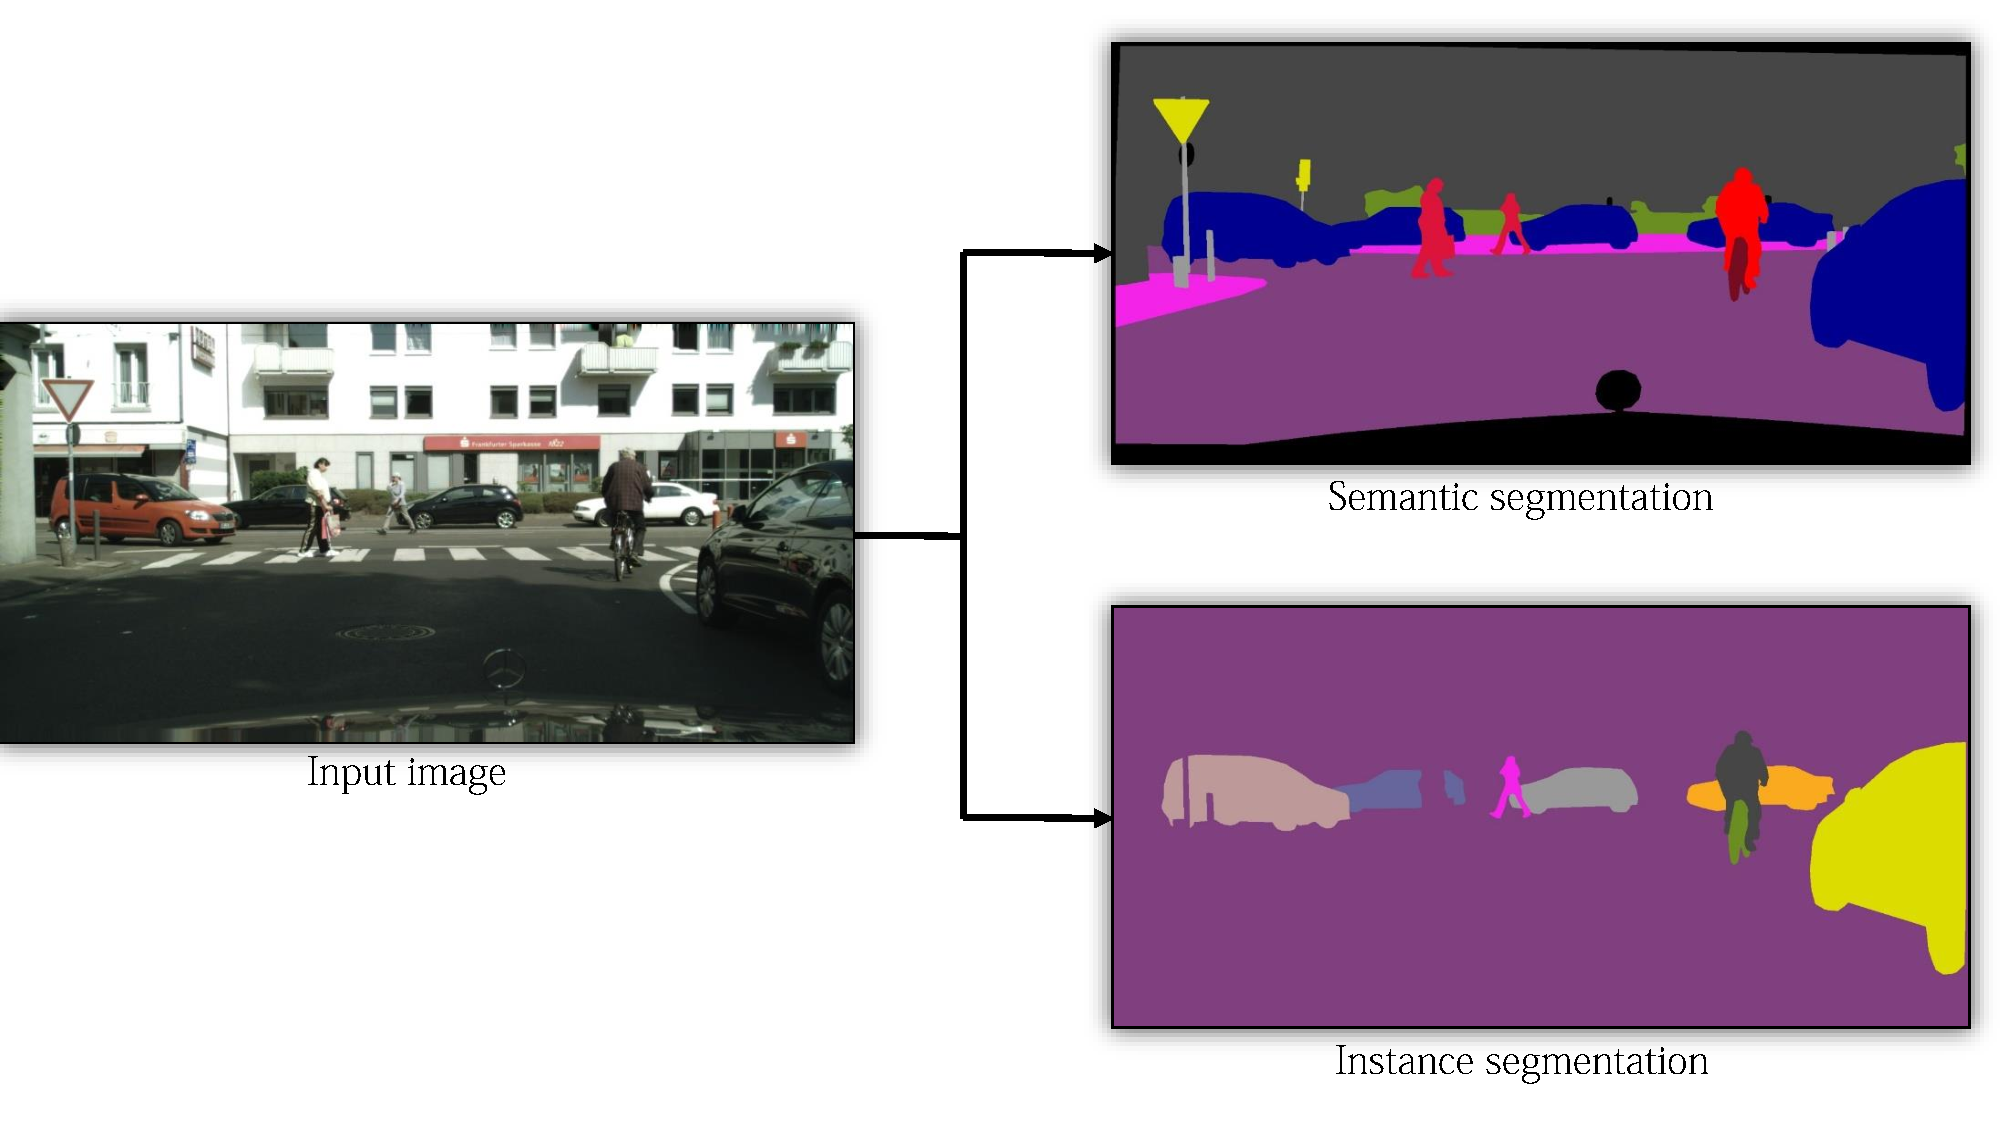
\includegraphics[width = \textwidth]{Graphics/Related_Work/SemInstImage.pdf}
    \caption[Semantic vs Instance Segmentation]{Illustration of an RGB Image taken from drivers perspective and its corresponding instance and semantic segmentation taken from Cityscapes Dataset \cite{Cordts2015}}
    \label{fig:rgb_instsemseg}
\end{figure}

\section{Panoptic Segmentation}

Panoptic segmentation aims to combine both of segmentation approaches described in former sections of this chapter. Very recently proposed panoptic segmentation task unifies the typically disjoint tasks of assigning class label to every pixel (\textit{semantic segmentation}) and detect and segment each object instance (\textit{instance segmentation}) \cite{Kirillov2019}, see figure \ref{fig:panoptic_seg} for reference.

\begin{figure}[!ht]
    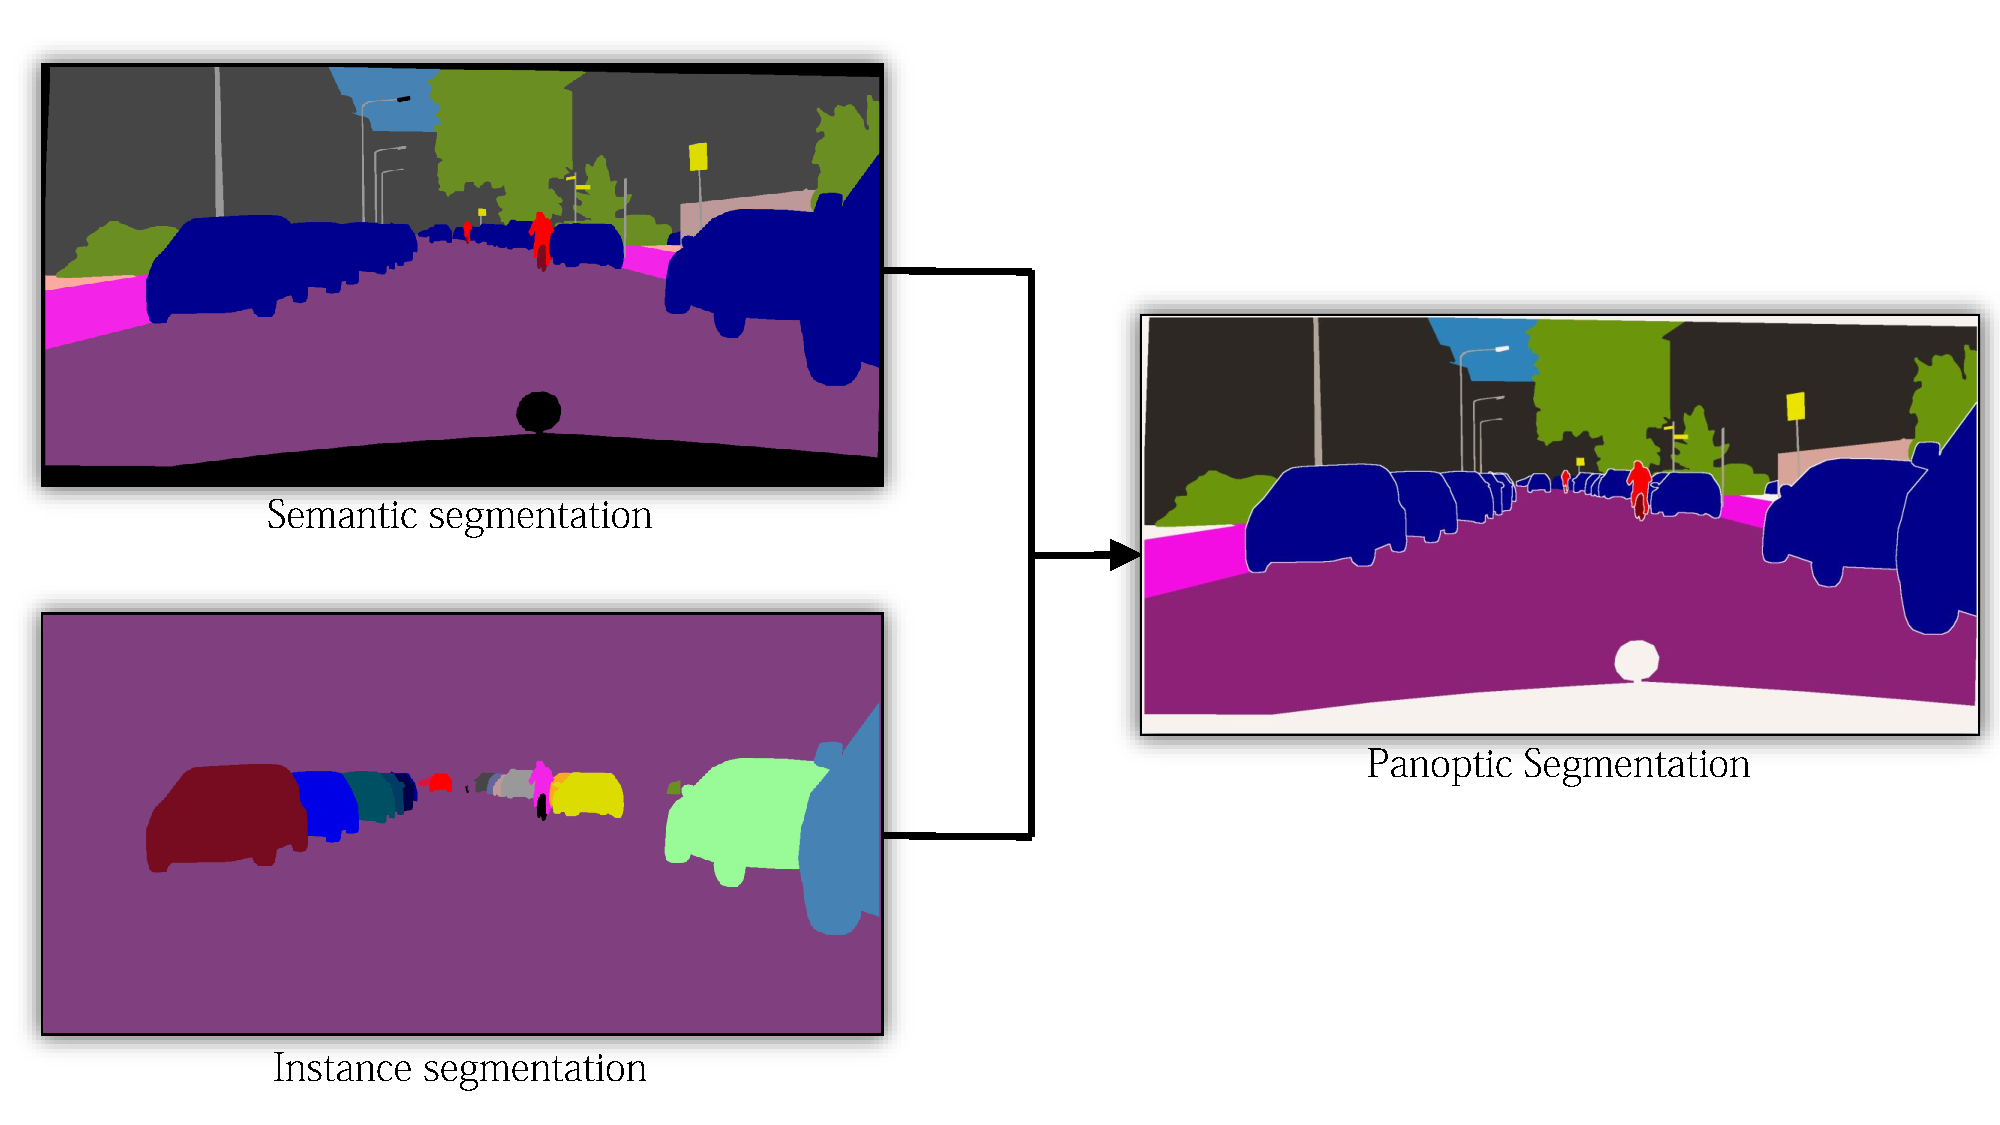
\includegraphics[width = \textwidth]{Graphics/Related_Work/PanopticSeg.pdf}
    \caption[Panoptic Segmentation]{Illustration of panoptic segmentation as a unified segmentation task -sample image taken from Cityscapes Dataset \cite{Cordts2015}}
    \label{fig:panoptic_seg}
\end{figure}


Numerous methods have been proposed for independent sub-tasks of panoptic segmentation, some of which have been briefly covered in the previous sections. However, there have been very few approaches that have tackled the task in a combined fashion. This section is dedicated to related literature review of state-of-the-art approaches that have been introduced for panoptic segmentation exclusively. 

Methods that address panoptic segmentation can be broadly classified into two
categories: 
\begin{itemize}
    \item Top-down or proposal based methods
    \item Bottom-up or proposal free methods
\end{itemize}


\subsection{Top-down approaches}

Most of the current state-of-the-art methods are top-down approaches. Panoptic segmentation task was proposed by \cite{Kirillov2019}, along with reviving the unified segmentation task, they also proposed a top-down baseline model based on PSPNet \cite{Zhao2017} and Mask R-CNN \cite{He2017}, for semantic segmentation and instance segmentation respectively. Joint training with a shared backbone that incorporates a Mask R-CNN type of architecture for instance segmentation, and augments a pyramid pooling module for semantic segmentation has been proposed by \cite{DBLPDaandeGues:journals/corr/abs-1809-02110}. An attention guided unified network that used proposal attention and mask attention module was proposed by \cite{Li2019} for joint segmentation task.
\textit{Unified Panoptic Segmentation Network} (UPSNet) introduces parameter free panoptic head to resolve conflicting and overlapping instances by prediciting an extra class. Subsequently, AdaptIS uses points to generate class agnostic instance masks and combines with semantic segmentation pipeline to perform panoptic segmentation \cite{adaptis2019}. More recently, \cite{Porzi2019} proposed an architecture that leverages novel segmentation head to integrates multi-scale features generated by a feature pyramid network (FPN) \cite{Lin2017} and conveyed using Deeplab-like \cite{Chen2018} module. 


Finally, \textit{Efficient panoptic segmentation architecture} (EfficientPS) is the current state-of-the-art at the time of writing this thesis \cite{mohan2020efficientps}. EfficientPS consists of a shared backbone that encodes and fuses multi-scale features. They propose a new semantic
head that aggregates features and propose a variant of Mask R-CNN as the instance head along-with a panoptic fusion module that integrates the output logits from both the heads to generate final panoptic output.

\subsection{Bottom-up approaches}

There have been very few bottom up, proposal free methods for panoptic segmentation. First bottom-up panoptic segmentation was \textit{Deeper-Lab}, that adopted bounding box corners as well as object center points for class-agnostic instance segmentation \cite{DBLPDeeperLab:journals/corr/abs-1902-05093}. Recently, \cite{Gao2019} proposed pixel grouping based on pixel-pair affinity pyramid \cite{Liu2018} with an efficient graph partition method \cite{Keuper2015}. Subsequently, \textit{panoptic-deeplab} was proposed as a solid baseline for bottom-up methods \cite{Cheng_2020_CVPR}. Panoptic-deeplab adopts the dual-\Gls{aspp} and dual-decoder structures specific to semantic and instance segmentation respectively. Semantic segmentation branch relies on typical design of deeplab \cite{Chen2018}, while instance segmentation branch adopts a simple instance center regression approach to generate class-agnostic instance masks. These instance masks are combined with semantic segmentation to generate panpotic segmentation. Presented work is majorly inspired by aforementioned proposal-free, bottom up panoptic segmentation architecture.  